\documentclass[a4paper,12pt]{article} % добавить leqno в [] для нумерации слева
\usepackage{comment}


\usepackage{hyperref}
\usepackage[rgb]{xcolor}
\hypersetup{
colorlinks=true,urlcolor=blue
}

\usepackage{geometry}
 \geometry{
 a4paper,
 total={170mm,257mm},
 left=15mm,
 right=15mm,
 top=10mm,
 bottom=20mm
 }

\usepackage{tabularx}


\usepackage{wrapfig}
\usepackage{graphicx}
\usepackage{mathtext}
\usepackage{amsmath}
\usepackage{siunitx} % Required for alignment
\usepackage{subfigure}
\usepackage{multirow}
\usepackage{booktabs}
\usepackage{rotating}

\usepackage{floatrow}
\restylefloat{table}

\usepackage[T1,T2A]{fontenc}
\usepackage[russian]{babel}
\usepackage{caption}

%%% Дополнительная работа с математикой
\usepackage{amsmath,amsfonts,amssymb,amsthm,mathtools} % AMS
\usepackage{icomma} % "Умная" запятая: $0,2$ --- число, $0, 2$ --- перечисление

%% Номера формул
\mathtoolsset{showonlyrefs=true} % Показывать номера только у тех формул, на которые есть \eqref{} в тексте.

%% Шрифты
\usepackage{euscript}	 % Шрифт Евклид
\usepackage{mathrsfs} % Красивый матшрифт
%\usepackage{txfonts}
%\usepackage{pxfonts}
\usepackage{caption}


%% Свои команды
\DeclareMathOperator{\sgn}{\mathop{sgn}}
\DeclareMathAlphabet\mathbfcal{OMS}{cmsy}{b}{n}

%\DeclareBoldMathCommand\bm{OMS}{cmsy}{b}{n}
\usepackage{bm}
\newcommand{\Equip}[3]{
	
	\item{ #1:} $\Delta = \pm #2\; #3$}
\newcommand{\equip}[1]{
	
	\item{ #1}}

\graphicspath{{./images/}}


\begin{document}
\begin{titlepage}
\begin{center}
{\large МОСКОВСКИЙ ФИЗИКО-ТЕХНИЧЕСКИЙ ИНСТИТУТ (НАЦИОНАЛЬНЫЙ ИССЛЕДОВАТЕЛЬСКИЙ УНИВЕРСИТЕТ)}
\end{center}
\begin{center}
{\large Физтех-школа аэрокосмических технологий}
\end{center}
\begin{figure}[H]
\centering

\includegraphics[scale=0.2]{MIPT.jpg}
\end{figure}

\vspace{3.0cm}
{\huge
\begin{center}
{\bf Вопрос по выбору}\\
«Генерация второй гармоники в нелинейном кристалле».
\end{center}
}
\vspace{4cm}
\begin{flushright}
{\LARGE Авторы:\\ Пазов Тенгиз, Б03-302 \\ Симухин Егор, Б03-302 \\ Кулиш Павел, Б03-302 \\ Плотников Данил, Б03-302}
\end{flushright}
\vspace{2.2cm}
\begin{center}
Долгопрудный, 2025 г.
\end{center}
\end{titlepage}

\newpage

\section{Введение}
Данный вопрос по выбору посвящён одному из нелинейных оптических эффектов, а именно: генерации второй гармоники (ГВГ). Этот эффект  позволяет преобразовывать инфракрасное излучение в видимое, или же из видимого диапазона переходить в область УФ излучения. Генерацию второй гармоники стало возможно пронаблюдать благодаря изобретению лазеров, и сегодня это явление активно применяется, например, в исследованиях по направлению лазерного термоядерного синтеза и для накачки титан-сапфировых лазеров. 

Цель работы - изучить теорию, описывающую явление генерации второй гармоники, экспериментально пронаблюдать данный эффект с помощью лазера и нелинейного кристалла йодата лития, а также убедиться в справедливости некоторых теоретических соотношений.

\section{Теоретическая справка}
\subsection*{Генерация второй гармоники, как нелинейно-оптический
процесс}
Распространение света в среде описывается уравнениями Максвелла, дополненными материальными уравнениями.

Поскольку уравнения Максвелла линейны(операции в уравнениях линейны) то при линейности материальных уравнений линейна и вся система уравнений в целом. Это
значит, что световые волны распространяются в среде независимо друг
от друга, т.е. выполняется принцип суперпозиции световых волн, лежащий в основе линейной оптики.

Но линейное материальное уравнение $\vec{P} = \alpha \vec{E}$ приближённо: оно
справедливо лишь при малых напряжённостях $\vec{E}$ , малых по сравнению с напряжённостями $E_a$ внутриатомных полей. Так, для оценки, напряжённость поля $E_a$ внутри атома водорода равна $E_H = \frac{e}{4 \pi \varepsilon_{0} r_{\text{н}}^{2}} = 5,2 \cdot 10^{11}$ В/м.

Для других атомных структур радиус, на котором находится внешний электрон, может быть на порядок больше. В связи с этим внутриатомное поле для них $E_a \sim 10^8 \div 10^9$ В/см.
%\divisionsymbol

Тогда как напряженность электрического поля Е в пучке света обычного источника значительно меньше(так, для солнечного излучения вблизи земной поверхности $\sqrt{\overline{E^2}} = 7,2$ В/см.

Для лазеров же, напряжённость электрического поля излучения превосходит напряжённость обычных пучков света на несколько порядков. К настоящему времени созданы лазеры, позволяющие получать напряжённости электрического поля порядка $10^8$ В/см. Такая напряжённость электрического поля уже сопоставима с внутриатомными полями. При распространении столь мощного светового пучка в среде оптические параметры среды становятся зависимыми от напряжённости электрического поля волны, материальное уравнение, связывающее поляризацию среды $\overline{P}$ с напряжённостью поля световой волны $\overline{E}$, становится нелинейным. В самом деле, действующее на атом среды электрическое поле световой волны вызывает смещение зарядов $x$, у атома появляется индуцированный дипольный момент. При этом на электрон в атоме действует сила внешнего поля $e \cdot E(t)$ и возвращающая сила $F$:
\begin{equation}
m \cdot \ddot{x}(t) = e \cdot E(t) + F
\end{equation}
При малых значениях интенсивности света, когда амплитуда колебаний электрона около положения равновесия мала, можно считать возвращающую силу квазиупругой силой:
\begin{equation}
F = -b \cdot x
\label{upr}
\end{equation}

Для гармонической световой волны $E(t) = E_0 \cdot \cos \omega t$ найдем решение в виде $X(t) = x_0 cos \omega t$.

Получается
\begin{equation}
X(t) = \frac{\frac{e}{m} E_0 \cos \omega t}{\omega^2_0 - \omega^2}
\end{equation}
Отсюда индуцированный дипольный момент атома
\begin{equation}
p(t) = e \cdot X(t) = \frac{\frac{e^2}{m} E_0 \cos \omega t}{\omega^2_0 - \omega^2}
\end{equation}

Тогда поляризация среды равна
\begin{equation}
P(t) = N \cdot p(t) = \frac{e^2 N E_0 \cos \omega t}{m(\omega^2_0 - \omega^2)}
\end{equation}
Где N - концетрация электронов с собственной частотой колебаний $\omega_0$.

Из этого соотношения видно
\begin{equation}
\alpha = \frac{e^2 N}{m(\omega^2_0 - \omega^2)}
\end{equation}
Поляризуемость среды не зависит от внешнего поля $E_0$ и определяет линейное материальное уравнение $\overline{P(t)} = \alpha \cdot \overline{E(t)}$

Однако данный результат может быть получен только если возвращающая сила $F$ подчиняется закону Гука $F(x) = -m \omega^2_0 x$. Но это имеет место лишь при не очень больших $x$. При больших $x$ имеет место отступление от закона Гука, колебания становятся нелинейными.

Функцию $F(x)$ в общем случае можно разложить в ряд Тейлора в окрестности точки равновесия $x=0$. Тогда 2 закон Ньютона для электрона записывается в ином виде
\begin{equation}
m \ddot{x} = eE + F(0) + F^{'}(0)x + \frac{F^{''}(0)}{2!}x^2 + \frac{F^{'''}(0)}{3!}x^3 + \ldots
\end{equation}
Поскольку точка $x = 0$ - равновесная, то $F(0) = 0$. Также при малых $x$, разложение должно соответствовать \eqref{upr}, поэтому $F^{'}(0) = -m \omega^2_0$. Тогда уравнение имеет вид
\begin{equation}
m \ddot{x} + m \omega^2_0 x = eE + \frac{F^{''}(0)}{2!}x^2 + \frac{F^{'''}(0)}{3!}x^3 + \ldots
\end{equation}
Если $F^{''}(0) \neq 0$, то нелинейность колебаний в первую очередь
проявляется за счёт члена, квадратичного по x. Тогда уравнение записывается в виде
\begin{equation}
m \ddot{x} + m \omega^2_0 x = eE + \frac{F^{''}(0)}{2!}x^2
\label{final_eq}
\end{equation}
Решив данное уравнение при помощи нулевого приближения(сначала находим $x(t)$ без нелинейного члена, затем подставляем это решение в это ангармоническое слагаемое, тем самым избавляемся от нелинейности), получим
\begin{equation}
x(t) = \frac{\frac{e}{m} E_0}{\omega^2_0 - \omega^2} \cos \omega t + \frac{F^{''}(0)}{4m\omega^2_0} \left[ \frac{\frac{e}{m} E_0}{\omega^2_0-\omega^2} \right]^2 + \frac{F^{''}(0)}{4m} \left[ \frac{\frac{e}{m} E_0}{\omega^2_0-\omega^2} \right]^2 \frac{\cos 2 \omega t}{\omega^2_0 - (2 \omega)^2}
\label{x}
\end{equation}
Колеблющийся оптический электрон является источником вторичных волн. Вынужденное движение электронов среды в поле световой волны макроскопически приводит к поляризации среды, складывающейся из дипольных моментов отдельных атомов. Из-за наличия ангармоничности в колебании электрона \eqref{final_eq} эти дипольные моменты, кроме линейного члена, пропорционального напряжённости электрического поля световой волны, содержат члены, пропорциональные более высоким степеням напряжённости электрического поля. Поэтому в сильных световых полях материальное уравнение, связывающее поляризацию среды с напряжённостью электрического поля, будет нелинейным
\begin{equation}
P_i = \sum_{k} \alpha_{ik}(\overline{E}) E_k
\end{equation}
где $\alpha_{ik}(\overline{E})$ - компоненты тензора поляризуемости.

Тензор поляризуемости $\alpha_{ik} (\overline{E})$ в первом приближении можно переписать в виде
\begin{equation}
\alpha_{ik}(\overline{E}) = \alpha_{ik} + \sum_j \chi_{ikj} E_j
\end{equation}
где $\alpha_{ik}$ - компоненты тензора линейной поляризуемости, а $\chi_{ikj}$ - компоненты тензора нелинейной поляризуемости.

В этом случае материальное уравнение имеет вид
\begin{equation}
P_i = \sum_k \alpha_{ik} E_k + \sum_k \sum_j \chi_{ikj} E_k E_j
\label{pol}
\end{equation}

Теперь рассмотрим распространение исходной волны частоты $\omega$ вдоль оси OZ

\begin{figure}[H]
\centering
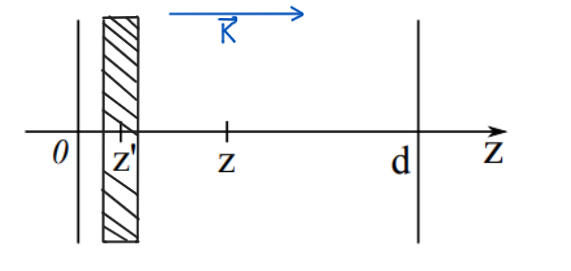
\includegraphics[scale=1]{pic1.png}
\caption{Интерференция вторичных волн при генерации второй гармоники}
\end{figure}

Тогда для диполей, расположенных в некоторой плоскости $z^{'}$, колебания с удвоенной частотой $2\omega$ описываются, в соответствии с \eqref{x} функцией
\begin{equation}
X^{(2\omega)}(t, z^{'}) = A^2 \cos 2 \left[ \omega t + \varphi (z^{'}) \right]
\label{X}
\end{equation}
Где фаза $\varphi(z^{'})$ определяется фазовой скоростью первичной волны с частотой $\omega$
\begin{equation}
\varphi(z^{'}) = - k z^{'} = - \frac{\omega}{c} n(\omega) z^{'}
\end{equation}
$n(\omega)$ - показатель преломления среды. Тогда \eqref{X} запишется как
\begin{equation}
X^{(2\omega)} = A^2 \cos 2 \omega \left[t - \frac{n(\omega)}{c} z^{'} \right]
\end{equation}
Колеблющийся по данному закону диполь излучает вторичную волну частотой $2\omega$. Добавку фазы вторичной волны в какой-либо точке $z$ внутри нелинейной среды можно вычислить
\begin{equation}
\frac{2 \omega n(2\omega) (z^{'} - z)}{c}
\end{equation}
Тогда фаза колебаний в точке z равна
\begin{equation}
\varphi(z) = 2 \omega \left[ t - \frac{n(\omega)}{c} z^{'} \right] - \frac{2 \omega n(2\omega)(z-z^{'})}{c} = 2 \omega \{ t - \frac{n(2\omega)}{c} z + \left[ n(2\omega) - n(\omega) \right] \frac{z^{'}}{c} \}
\label{phase}
\end{equation}
Полное поле на частоте $2\omega$ в точке z есть сумма вторичных, волн, испущенных диполями, расположенными между входной поверхностью среды и плоскостью $z$. Если показатели преломления $n(\omega)$ и $n(2\omega)$ одинаковые, то фаза \eqref{phase} не зависит от расположения излучающего диполя, соответственно все вторичные волны синфазны и амплитуда напряжённости $E^{2\omega}_0$ второй гармоники пропорциональна расстоянию z от входной плоскости.

Равенство показателей преломления называется условием пространственной синфазности и соответствует наибольшей интенсивности второй гармоники, генерируемой в данной нелинейной среде. 

В общем случае показатели преломления зависят от частоты, поэтому напряжённость волны удвоенной частоты можно найти как($E^{(2\omega)} \sim d = eX$(поле диполя), ищем поле, как суперпозицию полей всех вторичных волн)
\begin{equation}
E^{2\omega} = gA^2 \int^z_0 \cos \{ 2\omega \left[ t - n(2\omega) \frac{z}{c} \right] + 2 \omega \Delta n \frac{z^{'}}{c} \} dz^{'}
\end{equation}
Где g - коэффициент пропорциональности. Тогда получается
\begin{equation}
E^{(2\omega)} = gA^2 z \frac{\sin \{k_0(\omega) \Delta n z \}}{k_0(\omega) \Delta n z} \cdot \cos \{2\omega\left( t - \frac{n(\omega) + n(2\omega)}{2c}z \right) \}
\label{sec_garm}
\end{equation}  
Как видно из \eqref{sec_garm}, амплитуда второй гармоники содержит интерфереционный множитель $sinc \left( k_0(\omega) \Delta n z \right)$, который отражает частичное или полное гашение вторичных волн, испущенных в различных точках среды.

На рисунке \ref{garm} приведена зависимость $| A^{(2\omega)} |$ от координаты z.

\begin{figure}[H]
\centering
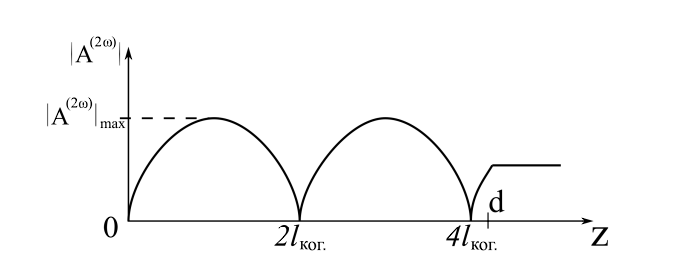
\includegraphics[scale=1]{pic2.png}
\caption{Зависимость амплитуды второй гармоники $| A^{(2\omega)} |$ от расстояния z}
\label{garm}
\end{figure}

Здесь $l_\text{ког} = \frac{\lambda}{4 \Delta n}$ - длина когерентности. Из рисунка видно, что при распространении волны происходят последовательные процессы накопления интенсивности второй гармоники и затем обратная перекачка энергии из волны $E^{(2\omega)}$ в волну $E^{(\omega)}$.

Если выполняется условие синхронизма $\Delta n = 0$, то длина когерентности $l_\text{ког}$ становится бесконечно большой.

Можно добиться выполнения условия фазового синхронизма, если применить в качестве нелинейной среды анизотропные кристаллы. Так, в одноосном кристалле на рисунке \ref{refl} показатель преломления для волны, поляризованной перпендикулярно оптической оси z кристалла (обыкновенная волна), $n_o$ не зависит от направления распространения волны. Для волны же, поляризованной в плоскости оптической оси (необыкновенная волна), зависимость показателя преломления $n_e$ от направления распространения достаточно сильная.

Одноосные кристаллы, для которых $n_e - n_o > 0$, называются положительными, а
кристаллы, для которых $n_e - n_o < 0$, называются отрицательными.

Если двупреломление $|n_e - n_o|$ велико, возможно пересечение эллипсоида $n_e(2\omega)$ и сферы $n_o(\omega)$, и в направлении $\Theta_0$ с оптической осью для отрицательных кристаллов $n_o(\omega) = n_e(2\omega)$

\begin{figure}[H]
\centering
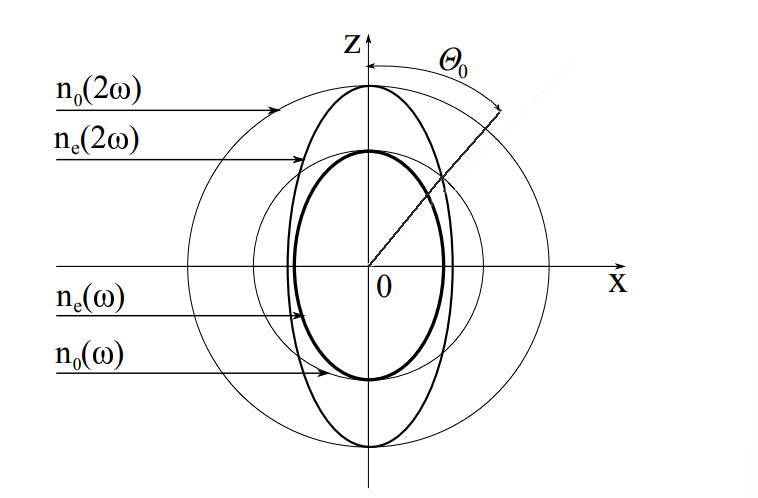
\includegraphics[scale=1]{pic3.png}
\caption{Сечения поверхностей показателя преломления обыкновенной $n_o(\omega), n_o(2\omega)$, и необыкновенной $n_e(\omega), n_e(2\omega)$ волн}
\label{refl}
\end{figure}

Таким образом, выполняется условие синхронизма, если основная волна обыкновенная, а волна второй гармоники - необыкновенная.

Угол $\Theta_0$ называется углом синхронизма. Его легко рассчитать, используя зависимость показателей преломлени от угла распространения луча:
\begin{equation}
n_o(\Theta) = const
\end{equation}
\begin{equation}
n_e(\Theta) = n_o \left[ 1 + \left(\frac{n^2_0}{n^2_e(\frac{\pi}{2})} - 1\right) \sin^2 \Theta \right]^{-\frac{1}{2}}
\end{equation}
Также важно отметить, что в реальном эксперименте когерентная длина не обращается в бесконечность при выполнении условия синхронизма, что связано с расходимостью световых пучков, приводящей к отклонению части лучей от направления синхронизма. Влияние расхождения пучка будем определять специальным параметром - градиентом рассогласования $\frac{d \Delta}{d \Theta}$.

Для примера на рисунке \ref{int} приведена зависимость интенсивности $I^{(2\omega)}(\Delta \Theta)$ второй гармоники в кристалле $LiNbO_3$ от угла между направлением распространения света $\Theta$ и направлением синхронизма $\Theta_0$.

\begin{figure}[H]
\centering
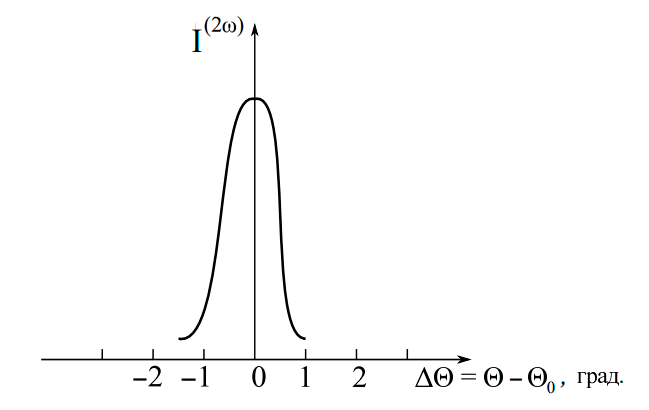
\includegraphics[scale=1]{pic4.png}
\caption{Зависимость интенсивности второй гармоники $I^{(2\omega)}$ от угла $\Delta \Theta$ в кристалле $LiNbO_3$}
\label{int}
\end{figure}

Согласно соотношению \eqref{sec_garm}, амплитуда $A^{(2\omega)}$ волны с удвоенной частотой пропорциональная квадрату амплитуды падающей волны A, а это значит, что интенсивность излучения волны второй гармоники пропорциональна квадрату интенсивности исходного пучка. Однако это имеет место только в случае, если $I^{(2\omega)}$ составляет небольшую часть от $I^{(\omega)}$, так как энергия второй гармоники, как было показано выше, черпается из первичной волны.
\subsection*{Тензор нелинейной восприимчивости $\chi_{ikj}$. \\Нелинейный кристалл $LiIO_3$}
Как было получено ранее, генерация второй гармоники определяется нелинейной поляризацией среды (cм. \eqref{pol})
\begin{equation}
P^{(2\omega)}_i = \sum_{j,k} \chi^{(2\omega)}_{ikj} E^{(\omega)}_j E^{(\omega)}_k
\label{2garm}
\end{equation}
где $\chi_{ijk}$ - тензор третьего ранга. Перестановка j и k не влияет на значение поляризации, получается имеет место симметрия
\begin{equation}
\chi^{(2\omega)}_{ijk} = \chi^{(2\omega)}_{ikj}
\end{equation}

Тогда данный тензор можно переписать в виде упрощённой матрицы(т.к. для каждому $i$ соответствуют 6, а не 9 различных значений, то матрица будет 3 на 6).

\begin{equation}
d_{im} = 1/2 \chi_{ikj}
\end{equation}
где
\begin{table}[H]
\begin{tabular}{c c c c c c c}
kj & 11 & 22 & 33 & 23, 32 & 31, 13 & 12, 21 \\
m & 1 & 2 & 3 & 4 & 5 & 6 \\
\end{tabular}
\end{table}

Тогда выражение \eqref{2garm} можно переписать в матричной форме
\begin{equation}
\begin{bmatrix}
P_x \\
P_y \\
P_z
\end{bmatrix}
= 
\begin{bmatrix}
d_{11} & d_{12} & d_{13} & d_{14} & d_{15} & d_{16} \\
d_{21} & d_{22} & d_{23} & d_{24} & d_{25} & d_{26} \\
d_{31} & d_{32} & d_{33} & d_{34} & d_{35} & d_{36}
\end{bmatrix}
\cdot
\begin{bmatrix}
E^2_x \\
E^2_y \\
E^2_x \\
2 E_y E_z \\
2 E_x E_z \\
2 E_x E_y
\end{bmatrix}
\label{mat}
\end{equation}
$d_{im}$ - тензор квадратичной нелинейной восприимчивости.

Число ненулевых членов в $d^{(2\omega)}_{im}$ зависит от группы точечной симметрии среды. Для применяемого кристалла иодата лития $LiIO_3$ (класс $6 - C_6$) данный тензор имеет вид
\begin{equation}
d_{im} =
\begin{bmatrix}
0 & 0 & 0 & d_{14} & d_{15} & 0 \\
0 & 0 & 0 & d_{15} & -d_{14} & 0 \\
d_{31} & d_{31} & d_{33} & 0 & 0 & 0
\end{bmatrix}
\end{equation}

Теперь, зная этот тензор для нашего случая, найдём чему равна интенсивность второй гармоники. Будет рассматривать такую первичную волну с частотой $\omega$, при которой выполняется условие синхронизма. Как уже было отмечено ранее, для этого падающая волна должна быть обыкновенной - её вектор напряженности $\vec{E^{(\omega)}}$ должен быть перпендикулярен оптической оси z. Пусть она распространяется в кристале под углом $\Theta$ к оптической оси z в плоскости, проходящей через оптическую ось и составляющей угол $\varphi$ с осью x (рисунок \ref{wave}).

\begin{figure}[H]
\centering
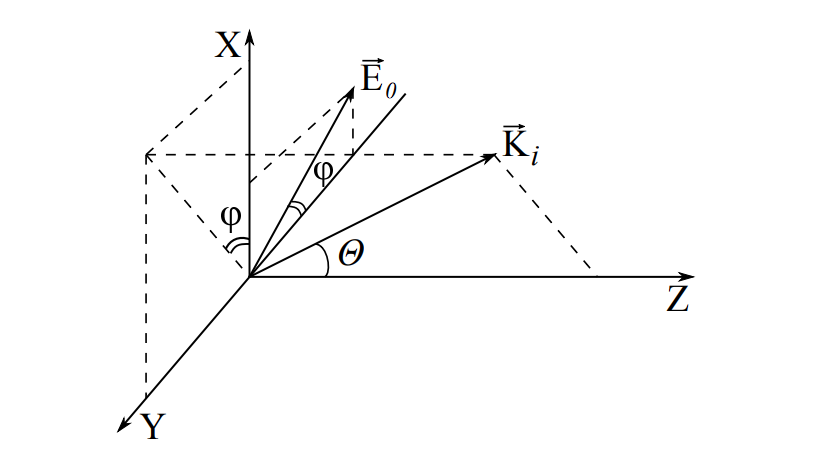
\includegraphics[scale=1]{pic5.png}
\caption{Распространение обыкновенной волны относительно осей кристалла}
\label{wave}
\end{figure}
Как видно из геометрии, проекции вектора $\vec{E}$ на оси координат($\vec{E}$ перпендикулярен $\vec{k}$, а также оптической оси, значит он перпендикулярен всей плоскости kZ, а значит также перпендикулярен проекции вектора $\vec{k}$ на плоскость xy)
\begin{equation}
E_x = E_o \sin \varphi \\
E_y = - E_o \cos \varphi \\
E_z = 0
\end{equation}
Тогда подставим в \eqref{mat}
\[P_y = 0\]
\begin{equation}
P_y = 0
\end{equation}
\[P_z = d_{31} (E^2_x +E^2_y)\]



Тогда компонента нелинейной поляризации, дающая необыкновенную волну, равна(с учётом, что поле необыкновенной волны должно лежать на главной плоскости)
\begin{equation}
P_e = P_z \sin \Theta
\end{equation}
Тогда в итоге, т.к. для колеблющихся диполей интенсивность задаётся формулой $I = \frac{2}{3c^3} |\ddot{P}|^2$, то интенсивность второй гармоники равна
\begin{equation}
I^{(2\omega)} = \frac{8 \omega^4}{3c^3} d^2_{31} \sin^2 \theta \left( I^{(\omega)} \right)^2
\label{int}
\end{equation}
и не зависит от угла $\varphi$

\section{Экспериментальная установка}
Схема установки представлена на рисунке \ref{scheme}.

\begin{figure}[H]
\centering
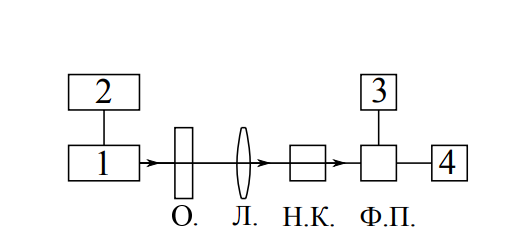
\includegraphics[scale=1]{pic6.png}
\caption{Схема установки для изучения второй гармоники}
\label{scheme}
\end{figure}
\begin{figure}[H]
\centering
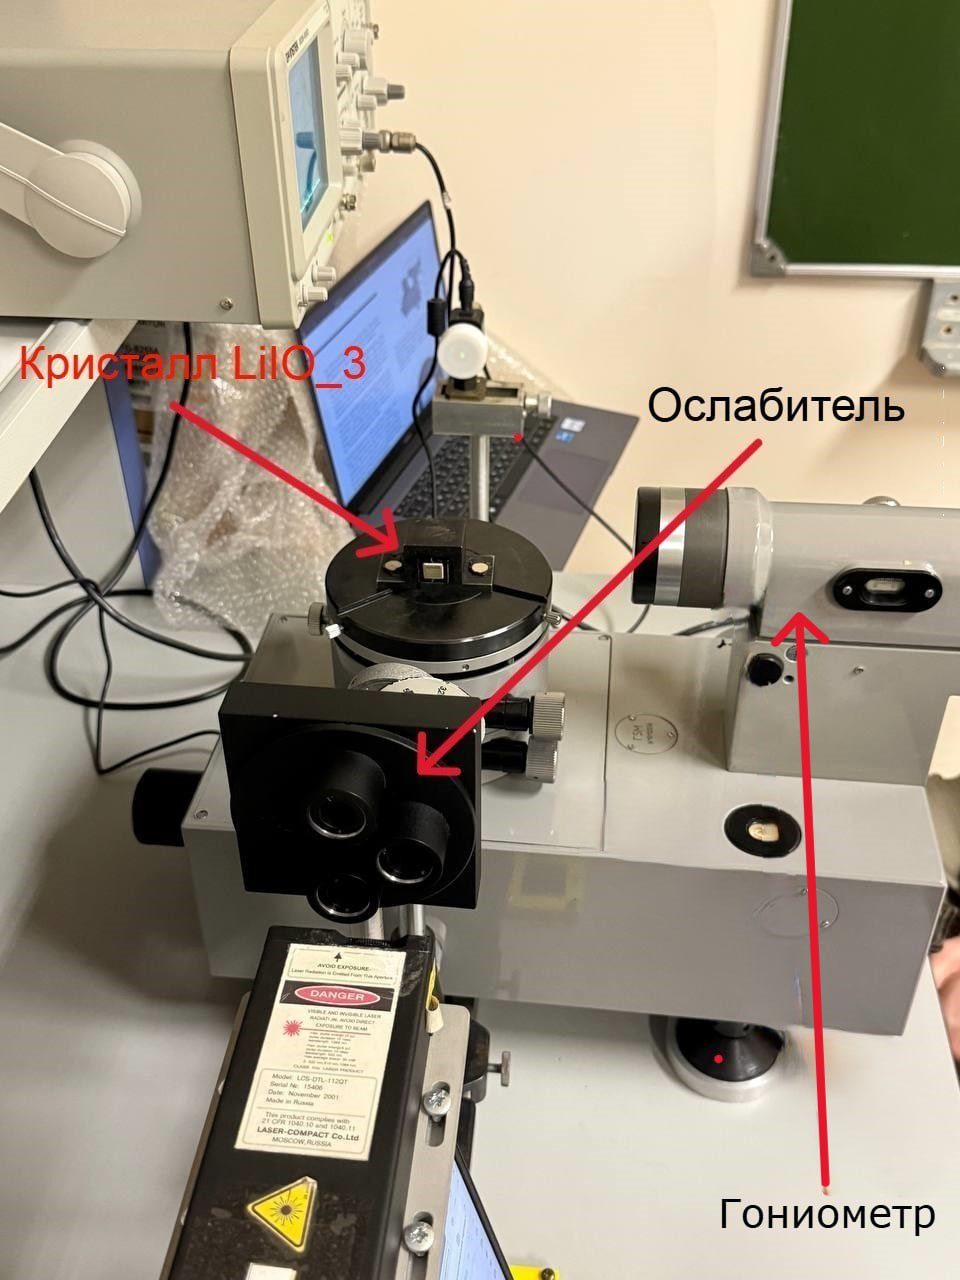
\includegraphics[scale=0.45]{goniometr.jpg}
\caption{Схема установки для изучения второй гармоники}
\label{scheme}
\end{figure}
Сигнал подаётся твёрдотельным лазером, который состоит из излучателя 1 и блока питания 2(работаем в режиме с длиной волны $\lambda = 1064$ нм). Далее сигнал проходит ослабитель О, который служит для изменения интенсивности излучения, и линзу-корректор Л., служащую для уменьшения расходимости пучка, выходящего из лазера, после чего попадает в нелинейный кристал Н. К., где его частота удваивается. Излучение удвоенной частоты далее попадает в фотоприёмник Ф.П(с блоком питания 3), с подключенным к нему осциллографом 4, который регистрирует интенсивность излучения.

Также для измерения изменения угла использовался гониометр, на который располагался нелинейный кристалл.

\section{Оборудование и инструментальные погрешности}

\begin{itemize}
\item Гониометр: в опыте по определению зависимости интенсивности второй гармоники от угла между направлением синхронизма и направлением распространения лазерного луча в качестве погрешности определения угла берётся значение 5 угловых секунд.
\end{itemize}
\section{Ход работы. Результаты измерений и обработка данных.}

\begin{enumerate}
\item Подготовим приборы к работе: отъюстируем гониометр, включим лазер, фотоприёмник и осциллограф.

\item Переведём излучение лазера на $\lambda = 1064 \; нм$: на экране осциллографа наблюдаем последовательность коротких импульсов. Поместив инфракрасный поляроид (ИП) на пути излучения лазера и повращав его, видим, что интенсивность излучения (смотрим на осциллограф) практически не изменяется. Таким образом, излучение лазера на этой длине волны имеет эллиптическую поляризацию. 

\item Проведём градуировку пропускания ослабителя О для излучения $\lambda = 1064 \; нм$: зарегистрируем интенсивность излучения при различных пропусканиях ослабителя $I = I(n)$, где $n$ - номер окна ослабителя. Данные занесены в таблицу \ref{I_532_1064}.


\begin{table}[htbp]
\caption{Градуировка пропускания ослабителя О для излучения $\lambda = 1064 \; нм$}
\begin{center}
\begin{tabular}{|c|c|c|c|}
\hline
n & $N, \; делений$ & $I$ & $Scale$\\ \hline
0 & 6.6 & 43.56 & 1\\ \hline
1 & 6.8 & 11.56 & 0.5\\ \hline
2 & 7.7 & 14.82 & 0.5\\ \hline
3 & 4.8 & 23.04 & 1\\ \hline
\end{tabular}
\end{center}
\label{I_532_1064}
\end{table}

\item Установим на столике гониометра наш нелинейный кристалл LiIO$_3$, и отрегулируем положение столика. В результате на поверхности тефлонового фильтра видим пятно зелёного цвета - произошла генерация второй гармоники ($\lambda = 532 \; нм$).

\item С помощью поляроида для видимого света (ВП) определим поляризацию второй гармоники. При вращении поляроида при определённом угле поворота на тефлоновом фильтре зелёное пятно практически не видно. Это означает, что поляризация второй гармоники  - линейная.

\item Поместим на фотоприёмнике зелёный фильтр. Теперь на экране осциллографа отображается только интенсивность второй гармоники. Слегка изменяя угол поворота кристалла и наблюдая картинку на экране осциллографа, добьёмся максимума интенсивности второй гармоники.
\begin{figure}[H]
\centering
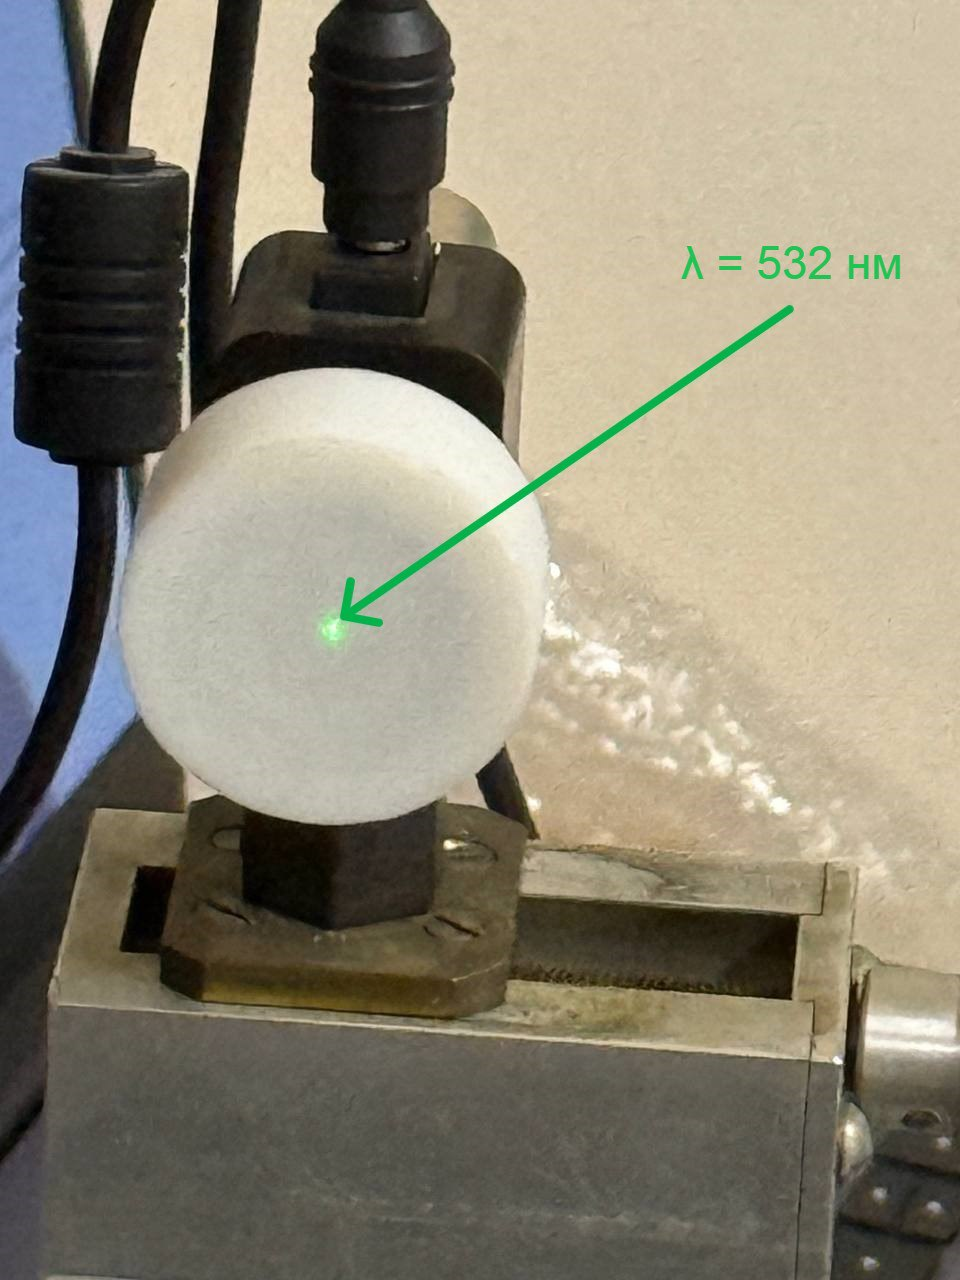
\includegraphics[scale=0.2]{generate2w.jpg}
\caption{Наблюдение второй гармоники}
\end{figure}

\item Воспользуемся градуированным ослабителем для нахождения зависимости интенсивности второй гармоники ($\lambda = 532 \; нм$) от интенсивности возбуждающей линии ($\lambda = 1064 \; нм$). Результаты трёх серий измерений приведены в таблице \ref{exp1}. Такое количество измерений связано с тем, что у нас всего 4 значения интенсивности исходного излучения, и четырёх точек может быть недостаточно для того, чтобы сделать вывод о соответствии эксперимента теории.


\begin{table}[H]
\caption{Зависимость интенсивности второй гармоники $I^{(2\omega)}$ от интенсивности исходного излучения $I^{(\omega)}$}
\begin{center}
\begin{tabular}{|c|c|c|c|c|}
\hline
№ опыта & $I_{1064}, \; В$ & $I_{532}, \; В$ & $\sigma_{1064}, \; В$ & $\sigma_{532}, \; В$ \\ \hline
\multirow{4}{*}{1} & 4.159 & -2.279 & 0,1 & 0,1 \\ \cline{2-5}
& 2.671 & -5.319 & 0,1 & 0,1 \\ \cline{2-5}
& 2.964 & -5.051 & 0,1 & 0,1 \\ \cline{2-5}
& 3.298 & -4.415 & 0,1 & 0,1 \\ \hline
\multirow{4}{*}{3} & 4.159 & -2.043 & 0,1 & 0,1 \\ \cline{2-5}
& 2.671 & -5.051 & 0,1 & 0,01 \\ \cline{2-5}
& 2.964 & -4.269 & 0,1 & 0,1 \\ \cline{2-5}
& 3.298 & -4.255 & 0,1 & 0,1 \\ \hline
\multirow{4}{*}{3} & 4.159 & -2.408 & 0,1 & 0,1 \\ \cline{2-5}
& 2.671 & -5.922 & 0,1 & 0,1 \\ \cline{2-5}
& 2.964 & -4.817 & 0,1 & 0,1 \\ \cline{2-5}
& 3.298 & -4.415 & 0,1 & 0,1 \\ \hline
\end{tabular}
\end{center}
\label{exp1}
\end{table}

Построим графики зависимостей $I_{532} = f (I_{1064})$ для каждой серии измерений в логарифмическом масштабе. Убедимся в том, что $I^{(2 \omega)} \sim (I^{(\omega)})^2$, как сказано в теории.

\begin{figure}[H]
	\label{graf_4}
	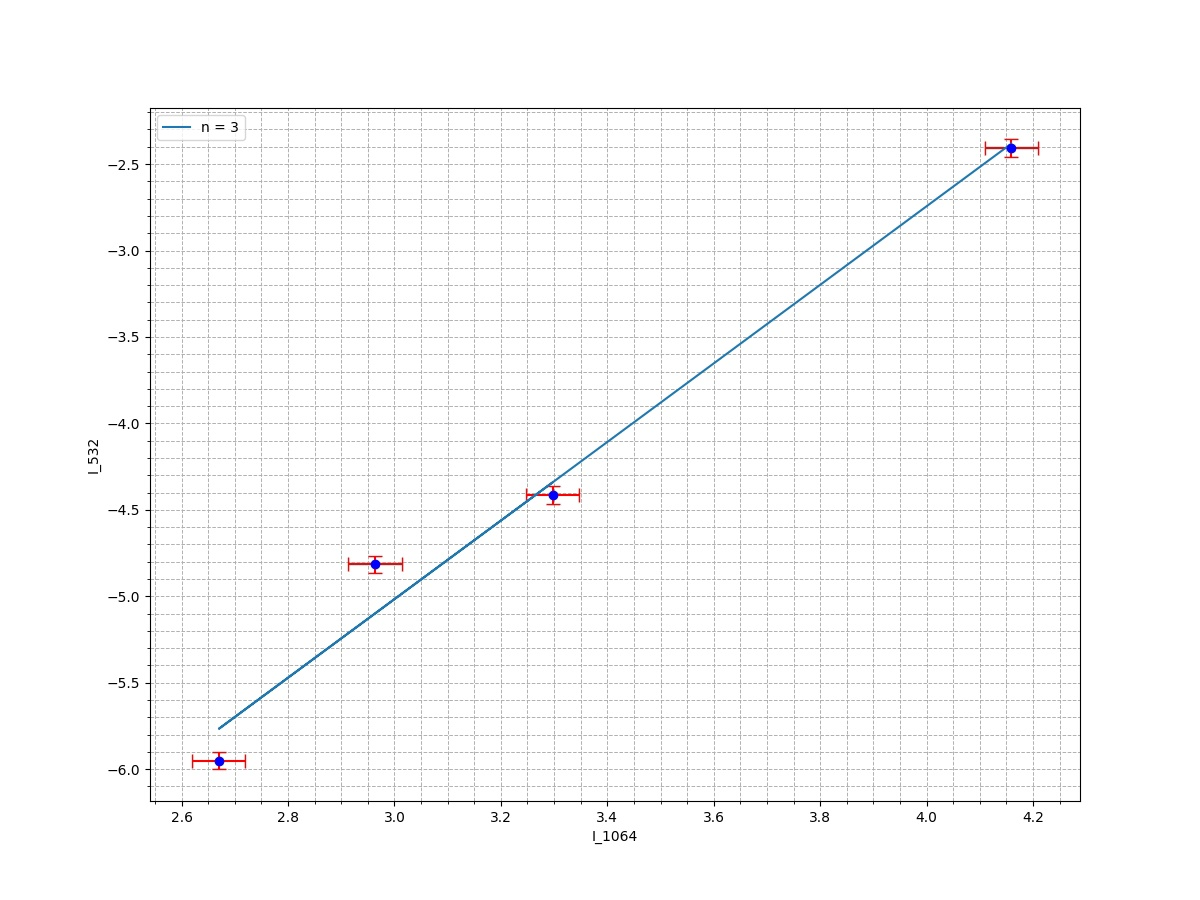
\includegraphics[scale=0.3]{1.jpg}
	\caption{Коэффициент наклона: $k = 1.96 \pm 0.21$}
\end{figure}

\begin{figure}[H]
	\label{graf_4}
	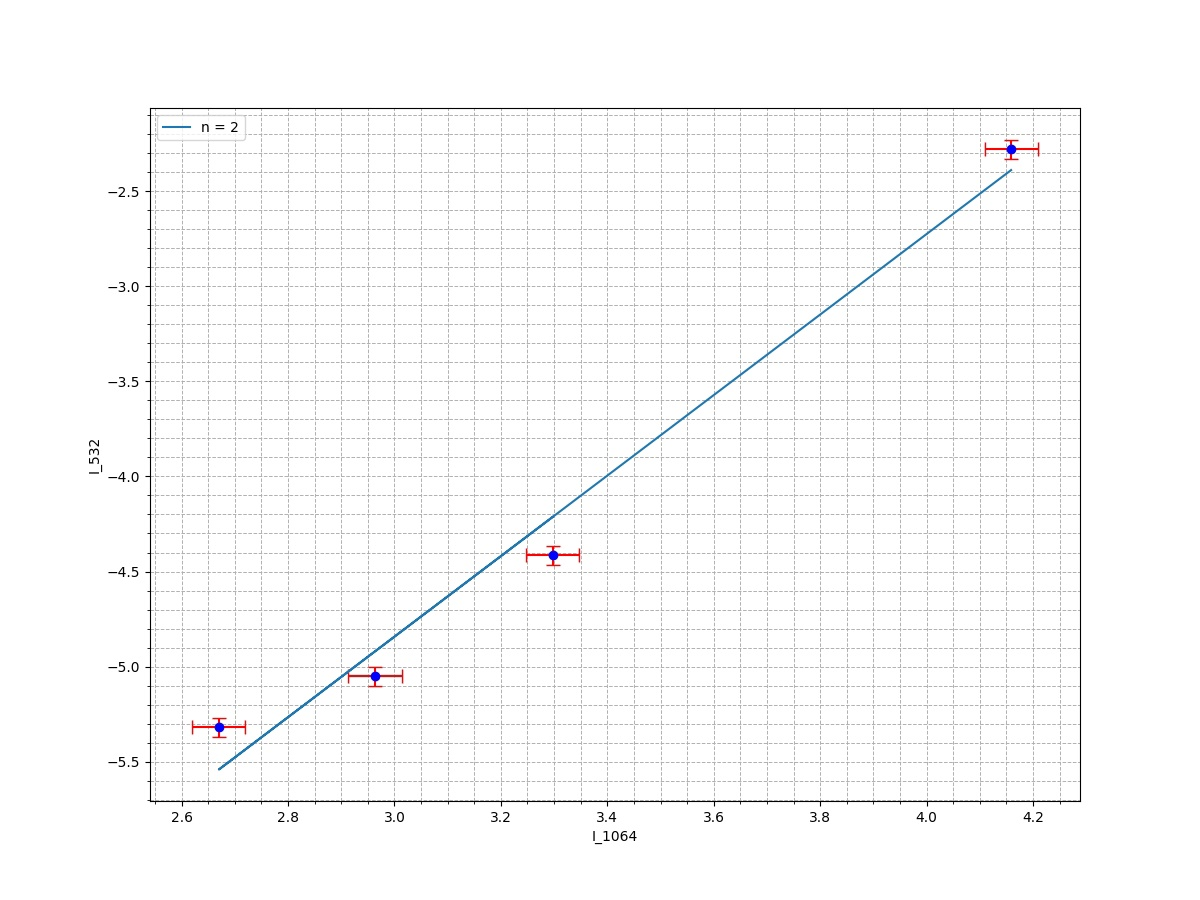
\includegraphics[scale=0.3]{2.jpg}
	\caption{Коэффициент наклона: $k = 2.11 \pm 0.15$}
\end{figure}

\begin{figure}[H]
	\label{graf_4}
	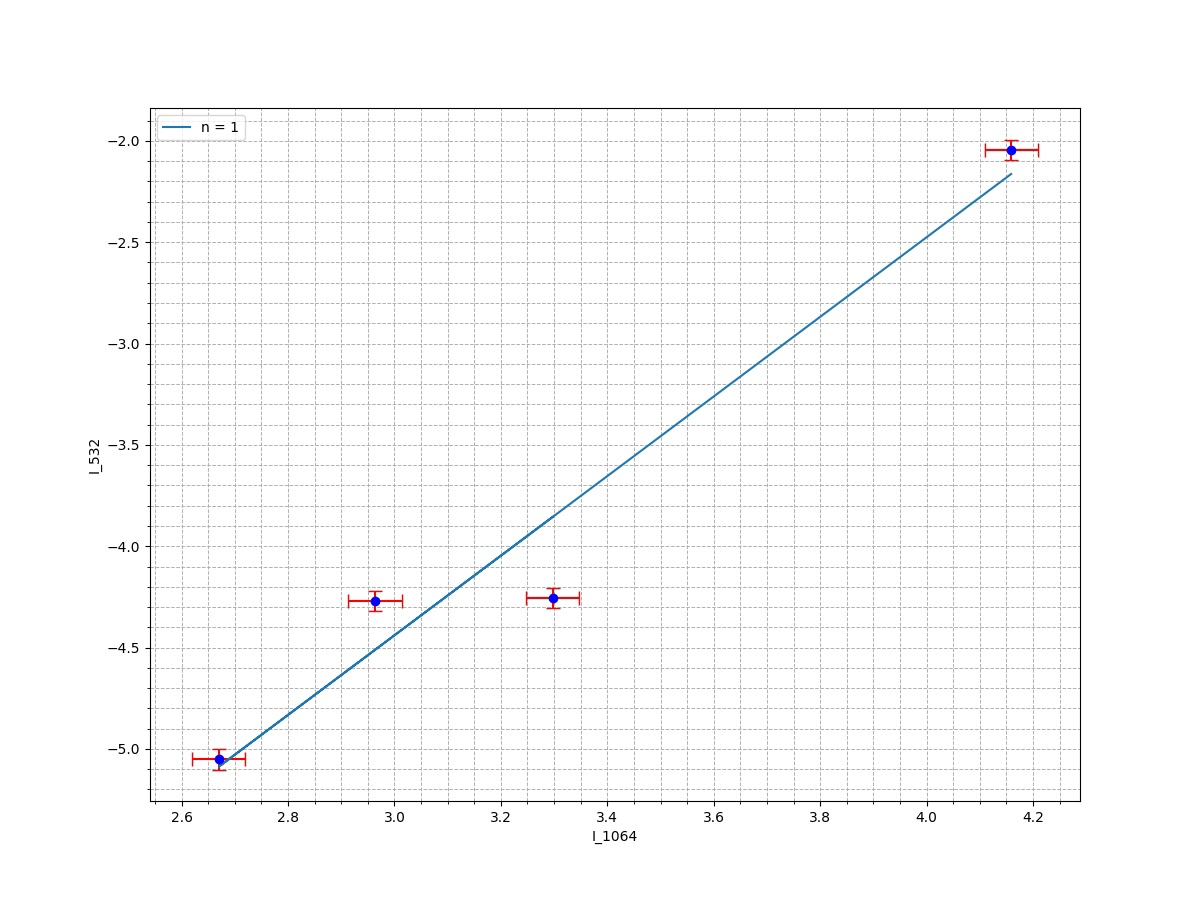
\includegraphics[scale=0.3]{3.jpg}
	\caption{Коэффициент наклона: $k = 2.27 \pm 0.15$}
\end{figure}

Как видно из графиков, коэффициент наклона прямой близок к значению 2. (В графиках 7 и 8 имеем $k = 2$ в пределах погрешности). Это означает, что формула \eqref{int} справедлива. Немалая погрешность
определения коэффициента наклона обусловлена наличием всего четырёх окон у ослабителя ( всего 4 точки на графике), а уход некоторых точек от прямой может быть связан с дефектами второго окна ослабителя (при незначительных сдвигах второго окна по отношению к лучу лазера высота импульсов на экране ЭО заметно колебалась).

\item С помощью гониометра найдём зависимость интенсивности второй гармоники от угла $\Delta \Theta = \Theta - \Theta_0$ между направлением распространения луча $\lambda = 1064 \; нм$ и направлением синхронизма. Построим график зависимости $I^{(2 \omega)} = f(\Delta \Theta)$ (см. рис. \ref{I_Dtheta}).


\begin{figure}[H]
	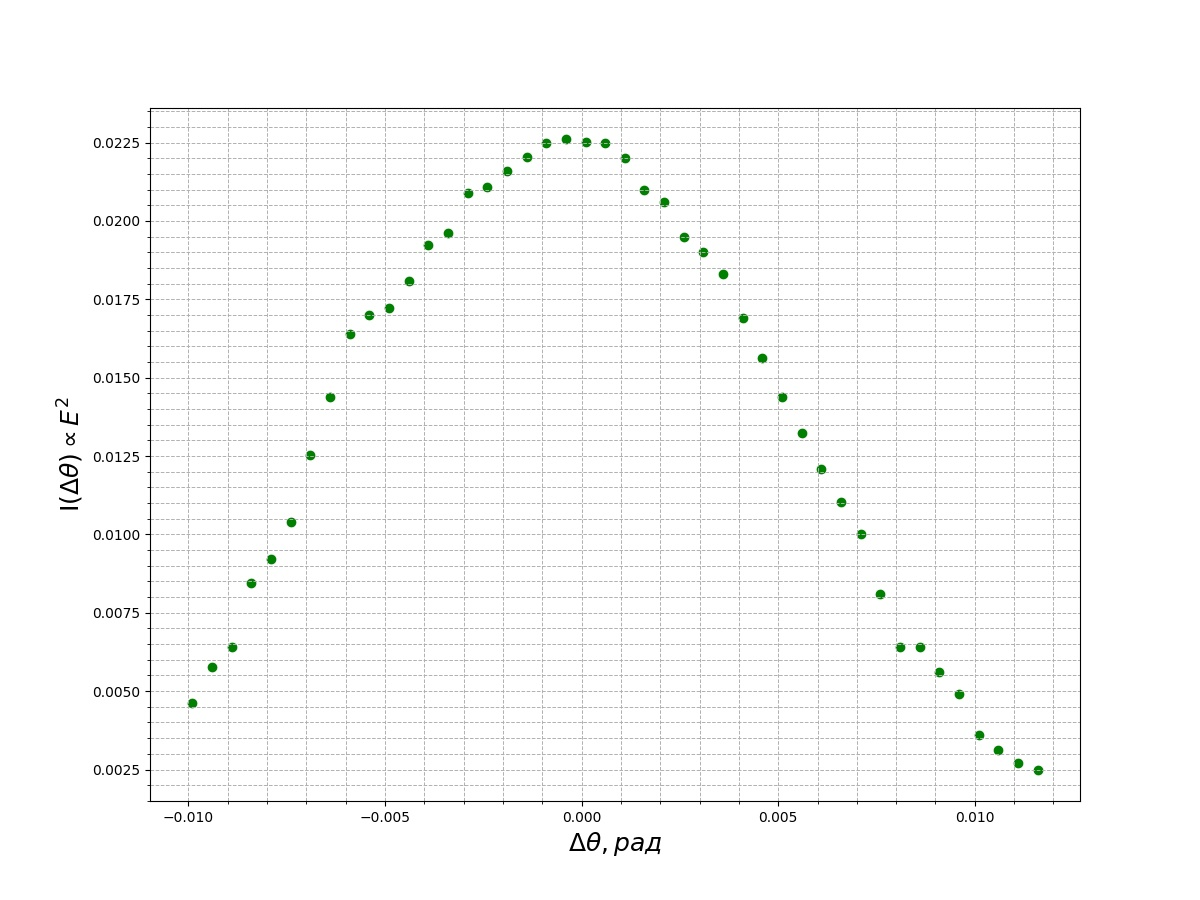
\includegraphics[scale=0.5]{4.jpg}
	\caption{График зависимости интенсивности второй грамоники $I^{(2 \omega)}$ от угла $\Delta \theta = \theta - \theta_0$ в исследуемом кристалле йодата лития}
	\label{I_Dtheta}
\end{figure}

Видим, что график такой зависимости для нашего кристалла качественно совпадает с графиком на рис. \ref{int} для ниобата лития.

\item Посчитаем коэффициент преобразования излучения лазера во вторую гармонику. Для этого измерим интенсивность возбуждающей линии, прошедшей через кристалл, в случае, когда излучение второй гармоники максимально и в случае, когда излучение $\lambda = 532 \; нм$ практически отсутствует (этого можно добиться поворотом кристалла). Разница двух интенсивностей $\Delta I(\omega)$ равна энергии, преобразованной во вторую гармонику. Таким образом, коэффициент преобразования равен:
$$K = \frac{\Delta I(\omega)}{I(\omega)} = \frac{4,9 - 4,4}{5} = 0,1 = 10 \%$$

\end{enumerate}

\section{Обсуждение результатов и выводы}
В ходе данного впв было исследовано явление генерации второй гармоники в кристале $LiIO_3$, а также были получены зависимости интенсивности генерируемого сигнала от интенсивности исходного, а также как зависит интенсивность второй гармоники от угла синхронизма.

\end{document}